

A distributed system is not just isolated instances of your applications running unaware of the existing world. They constantly communicate with each other and have to be properly integrated together to provide the most value.

Much was already said on the topic of integration, so in this section, we'll try to showcase just a handful of patterns for effective integration of both entirely new systems, as well as new parts of the system that needs to coexist with other existing parts, often legacy ones.

To not make this chapter be a whole book on its own, let's start this section with a recommendation of an existing one. If you're interested in integration patterns, especially focused on messaging, then Gregor Hohpe and Bobby Woolf's Enterprise Integration Patterns book is a must-read for you.

Let's take a brief look at two patterns covered by this book.


\subsubsubsection{4.4.1\hspace{0.2cm}管道与过滤器模式}

The first integration pattern that we'll discuss is called \textbf{pipes and filters}. Its purpose is to decompose a big processing task into a series of smaller, independent ones (called filters), which you can then connect together (using pipes, such as message queues). This approach gives you scalability, performance, and reusability.

Assume you need to receive and process an incoming order. You can do it in one big module, so you don't need extra communication, but the different functions of such a module would be hard to test and it would be harder to scale them well.

Instead, you can split the order processing into separate steps, each handled by a distinct component: one for decoding, one for validating, another one for the actual processing of the order, and then yet another one for storing it somewhere. With this approach, you can now independently perform each of those steps, easily replace or disable them if needed, and reuse them for processing different types of input messages.

If you want to process multiple orders at the same time, you can also pipeline your processing: while one thread validates a message, another thread decodes the next one, and so on.

The downside is that you need to use synchronized queues as your pipes, which introduces some overhead.

To scale one step of your processing, you might want to use this pattern along with the next one on our list.

\subsubsubsection{4.4.2\hspace{0.2cm}竞争消费者}

The idea of competing consumers is simple: you have an input queue (or a messaging channel) and a few instances of consumers that fetch and process items from the queue concurrently. Each of the consumers can process the message, so they compete with each other to be the receiver.

This way, you get scalability, free load balancing, and resilience. With the addition of the queue, you now also have the queue-based load leveling pattern in place.

This pattern integrates effortlessly with priority queues if you need to shave latency from a request or just want a specific task submitted to your queue to be performed in a more urgent manner.

\begin{tcolorbox}[colback=blue!5!white,colframe=blue!75!black, title=Note]
\hspace*{0.7cm}This pattern can get tricky to use if the ordering is important. The order in which your consumers receive and finish to process messages may vary, so make sure that either this doesn't impact your system, or you find a way to reorder the results later on. If you need to process messages in sequence, you might not be able to use this pattern.
\end{tcolorbox}

Let's now see a few more patterns, this time to help us integrate with existing systems.

\subsubsubsection{4.4.3\hspace{0.2cm}从遗留系统的过渡}

Developing a system from scratch can be a blissful experience. Development instead of maintenance and a possibility to use a bleeding-edge technology stack – what's not to like? Unfortunately, that bliss often ends when integrating with an existing, legacy system starts. Fortunately, though, there are some ways to ease that pain.

\hspace*{\fill} \\ %插入空行
\noindent
\textbf{防腐层}

Introducing an \textbf{anti-corruption layer} can help your solution in painless integration with a legacy system that has different semantics. This additional layer is responsible for communication between those two sides.

Such a component allows your solution to be designed with more flexibility – without the need to compromise your technology stack nor architectural decisions. To achieve that requires only a minimal set of changes in the legacy system (or none, if the legacy system doesn't need to make calls to the new system).

For instance, if your solution is based on microservices, the legacy system can just communicate with the anti-corruption layer instead of locating and reaching each microservice directly. Any translations (for example, due to outdated protocol versions) are also done in the additional layer.

Keep in mind that adding such a layer can introduce latency and has to satisfy quality attributes for your solution, for example, scalability.

\hspace*{\fill} \\ %插入空行
\noindent
\textbf{扼杀者模式}

The \textbf{strangler pattern} allows the gradual migration from a legacy system to a new one. While the anti-corruption layer we just looked at is useful for communication between the two systems, the strangler pattern is meant for providing services from both to the outside world.

Early in the migration process, the strangler facade will route most of the requests into the legacy system. During the migration, more and more calls can be forwarded into the new one, while strangling the legacy system more and more, limiting the functionality it offers. As the final step of the migration, the strangler, along with the legacy system, can be retired – the new system will now provide all the functionality:

\begin{center}
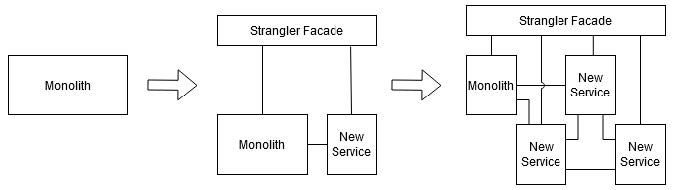
\includegraphics[width=0.9\textwidth]{content/2/chapter4/images/1.jpg}\\
Figure 4.1 – The strangling of a monolith. After the migration, the strangler can still be used as an entry point, or adapter, for legacy requests
\end{center}

This pattern can be overkill for small systems and can get tricky if the datastore should be shared or is for event-sourced systems. When adding it to your solution, be sure to plan for achieving the proper performance and scalability.

Speaking of those two attributes, let's now discuss a few things that help achieve them.















